\documentclass[a4paper, 12pt]{article}
\usepackage{matnoble-doc-en}


\begin{document}

\title{\bf {CHEM400/740: Quantum Mechanics in Chemistry\\ Chapter\#05: Derivation Hartree-Fock Equation}} \author{\bf
  \href{http://scienide2.uwaterloo.ca/~nooijen/website_new_20_10_2011/About.html}{Marcel Nooijen}} \date{}
  
\pagestyle{fancy} \fancyhead[L]{\textcolor{PrimaryColor}{CHEM400/740: Quantum Mechanics in Chemistry}} \fancyhead[R]{\textcolor{PrimaryColor}{2021 Winter}}


\maketitle
\tableofcontents

\clearpage


\section{Hartree-Fock Theory in a Finite Basis}

Hartree-Fock approximates the wave function by a single determinant, and optimizes the orbitals in the determinant to minimize energy, $\langle \phi_{HF}|\hat{H}|\phi_{HF} \rangle /\langle \phi_{HF}| \phi_{HF} \rangle $. The Hartree-Fock energy is greater than exact energy, $E_{HF}\geqslant E_{FCI}$.\\
\tab If we denote the occupied spin orbitals in $|\phi_{HF}\rangle$ by labeling $a,b$, then following the Slater rule.
	\begin{IEEEeqnarray}{rLl}
E_{HF} = \sum_{occ} \langle a|\hat{h}|b \rangle + \frac{1}{2}\sum_{a,b} \langle ab||ab \rangle 
	\end{IEEEeqnarray}
\tab NOTE:\\
\tab\tab 1. Anti-symmetrized two-electron integral: $\sum_{a>b}\langle ab||ab\rangle = \frac{1}{2}\sum_{a,b}\langle ab||ab \rangle$\\
\tab\tab\quad True because $\langle ba||ba\rangle =\langle ab||ab\rangle$. \\
\tab\tab 2. One-electron integral: $\sum_{occ} \langle a|\hat{h}|b \rangle$.

To minimize this expression I assume the HF spin-orbitals can be expressed in a basis set of spin orbital, $|\mu\rangle$, (AO's) that will carry greek indices for atomic orbital basis, $\mu,\nu,\sigma,\tau $. \\
\tab At this moment, I will do everything in terms of spin-orbitals. The AO basis set (or better primitive) basis set is given, and does not change. We need the following integrals. 
	\begin{IEEEeqnarray}{rLl}
\langle \mu|\hat{h}|\nu \rangle = h_{\mu\nu} &= \int \chi_\mu^*(1)\hat{h}_1\chi_{\nu}(1) d1 \\
\langle \mu \nu|\sigma\tau \rangle &=  \int \chi_\mu^*(1) \chi_\nu^*(2) \frac{1}{r_{12}} \chi_\sigma(1) \chi_\tau (2)d1d2 \\
S_{ \mu \nu} = \langle \mu|\nu \rangle &=\int \chi_\mu^*(1)\chi_\nu(1)d1
	\end{IEEEeqnarray}
\tab NOTE:\\
\tab \tab 1. The overlap integrals $S_{\mu\nu}$ are relevant because the primitive basis is non-orthogonal (e.g. AO-basis). AO integrals are not orthogonal in general.\\
\tab \tab 2. $\langle \mu \nu||\sigma\tau \rangle = \langle \mu \nu|\sigma\tau \rangle-\langle \mu \nu|\tau\sigma \rangle$.\\
\tab\tab\quad $\langle \mu \nu||\sigma\tau \rangle$ are the anti-symmetrized, including spin; $\langle \mu \nu|\sigma\tau \rangle$ are the primitive integrals.

The MO's can be expressed in the basis: 
	\begin{IEEEeqnarray}{rLl}
|a\rangle =\sum_{\mu}|\mu\rangle C_{\mu a}
	\end{IEEEeqnarray}

The MO's are supposed to be orthonormal.
	\begin{IEEEeqnarray}{rLl}
\delta_{ab} &= \langle b|a \rangle \notag \\
&= \sum_{\nu,\mu} C^*_{\nu b} \langle \nu|\mu\rangle C_{\mu a} \notag  \\
&= \sum_{\nu,\mu} C^*_{\nu b}S_{\nu\mu} C_{\mu a} \notag \\
&=  \sum_{\nu,\mu} (C^\dagger)_{n \nu} S_{\nu\mu} C_{\mu a} \\
&\Rightarrow C^\dagger SC=1
	\end{IEEEeqnarray}
\tab NOTE:\\
\tab\tab 1. $ C_{\mu a} $ and $C_{\nu b}$ represent MO coefficients from AO $*$ occupied MO matrix.\\
\tab\tab 2. $|b\rangle = \sum_\nu |\nu\rangle C_{\nu b} $ $\Rightarrow \langle b|=\sum_\nu \langle \nu|C^*_{\nu b}$\\
\tab\tab \quad $|a\rangle =\sum_\mu |\mu\rangle C_{\mu a}  $\\
\tab\tab 3. Transpose and take the Hermitian conjugate: $(C^\dagger )_{b \nu} = C^*_{\nu b}$.\\
\tab\tab 4. Natural order matrix multiply: $ \sum_{\nu,\mu} (C^\dagger)_{n \nu} S_{\nu\mu} C_{\mu a}$

Let us next consider the energy expression for a single determinant of orthonormal orbitals.
	\begin{IEEEeqnarray}{rLl}
E &= \sum_a \langle a|h|a\rangle +\frac{1}{2}\sum_{a,b}\langle ab||ab\rangle \notag \\
&= \sum_{\mu,\nu,a,occ} C^*_{\mu a} \langle \mu|h|\nu\rangle C_{\nu a} + \frac{1}{2}\sum_{a,b,occ}\sum_{\mu,\nu,\sigma,\tau}C^*_{\mu a}C^*_{\nu b}\langle \mu\nu||\sigma\tau\rangle C_{\sigma a}C_{\tau b}
	\end{IEEEeqnarray}
\tab NOTE:\\
\tab\tab 1. Always use different labels for each summation label.\\
\tab\tab \quad Name is irrelevant, but type for AO VS MO is important.

Next, define the (one-particle) density matrix: 
	\begin{IEEEeqnarray}{rLl}
D_{\nu\mu} = \sum_{a,occ} C^*_{\mu a} C_{\nu a} = \sum_{a,occ} C_{\nu a} (C^\dagger )_{a\mu} =(CC^\dagger )_{\nu\mu}
	\end{IEEEeqnarray}
\tab Similarly, $\sum_a C^*_{\mu a}C_{\sigma a} = D_{\sigma \mu}$; $\sum_{b}C^*_{\nu b}C_{\tau b} = D_{\tau \nu}$, where $a$ and $b$ are summation labels.

Then, the energy expression simplifies:
	\begin{IEEEeqnarray}{rLl}
E_{HF} &= \sum_{\mu,\nu} h_{\mu \nu} D_{\nu \mu} + \frac{1}{2}\sum_{\mu,\nu,\sigma,\tau}\langle \mu\nu||\sigma\tau\rangle D_{\sigma \mu}D_{\tau \nu}
	\end{IEEEeqnarray}
\tab The energy of a single determinant depends quadratically on the density matrix, $D_{\nu \mu}$.

\subsection{Property of Density Matrix}
Let us now show a fundamental property: \\
\tab The molecular orbitals are not unique. Define a new molecular orbital, which is the linear combination of old molecular orbitals. One can `rotate' the occupied orbitals among themselves; this does not affect the density matrix.
	\begin{IEEEeqnarray}{rLl}
|i\rangle = \sum_{\mu}C_{\mu i} =\sum_a |a\rangle u_{ai} \\
C_{\mu i} =\sum_a C_{\mu a} u_{a i}
	\end{IEEEeqnarray}
\tab where $u$ is a unitary matrix, $u^\dagger u =uu^\dagger =1$.
	\begin{IEEEeqnarray}{rLl}
D_{\mu\nu}^{(i)} &= \sum_i C_{\mu i}C_{\nu i}^* \notag \\
&= \sum_{a,b,i}(C_{\mu a} u_{ai})(C_{\nu b}^* u_{bi}^*) \notag \\
&= \sum_{a,b} C_{\mu a}C_{\nu b}^* \delta_{ab} \notag \\
&= \sum_{a} C_{\mu a}C_{\nu b} \notag \\
&\equiv D_{\mu\nu}^{(a)}
	\end{IEEEeqnarray}
\tab Hence, the energy is invariant under rotation of occupied orbitals. Also, the Slater determinants are the same, and up to a sign, $|\psi_a\psi_b \cdots| = sign \cdot |\psi_i\psi_j\cdots|$.\\
\tab Important: Only the density matrix matters, not the individual molecular orbitals. Determinant matters, not orbitals.

\begin{itemize}
\item Example for orbitals of water: \\
\tab $sp_3$ hybridization orbitals.
\begin{figure}[H]
        \centering
        % 1
        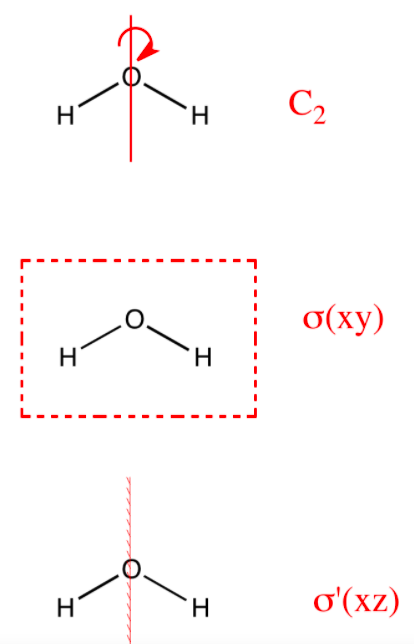
\includegraphics[width=.9\linewidth]{01.PNG}
        \caption{Orbitals for Water}
        \label{fig:sub-first2}
\end{figure}
Similar to methane, $CH_4$

Useful to construct Hydrogen-bondings:
\begin{figure}[H]
        \centering
        % 1
        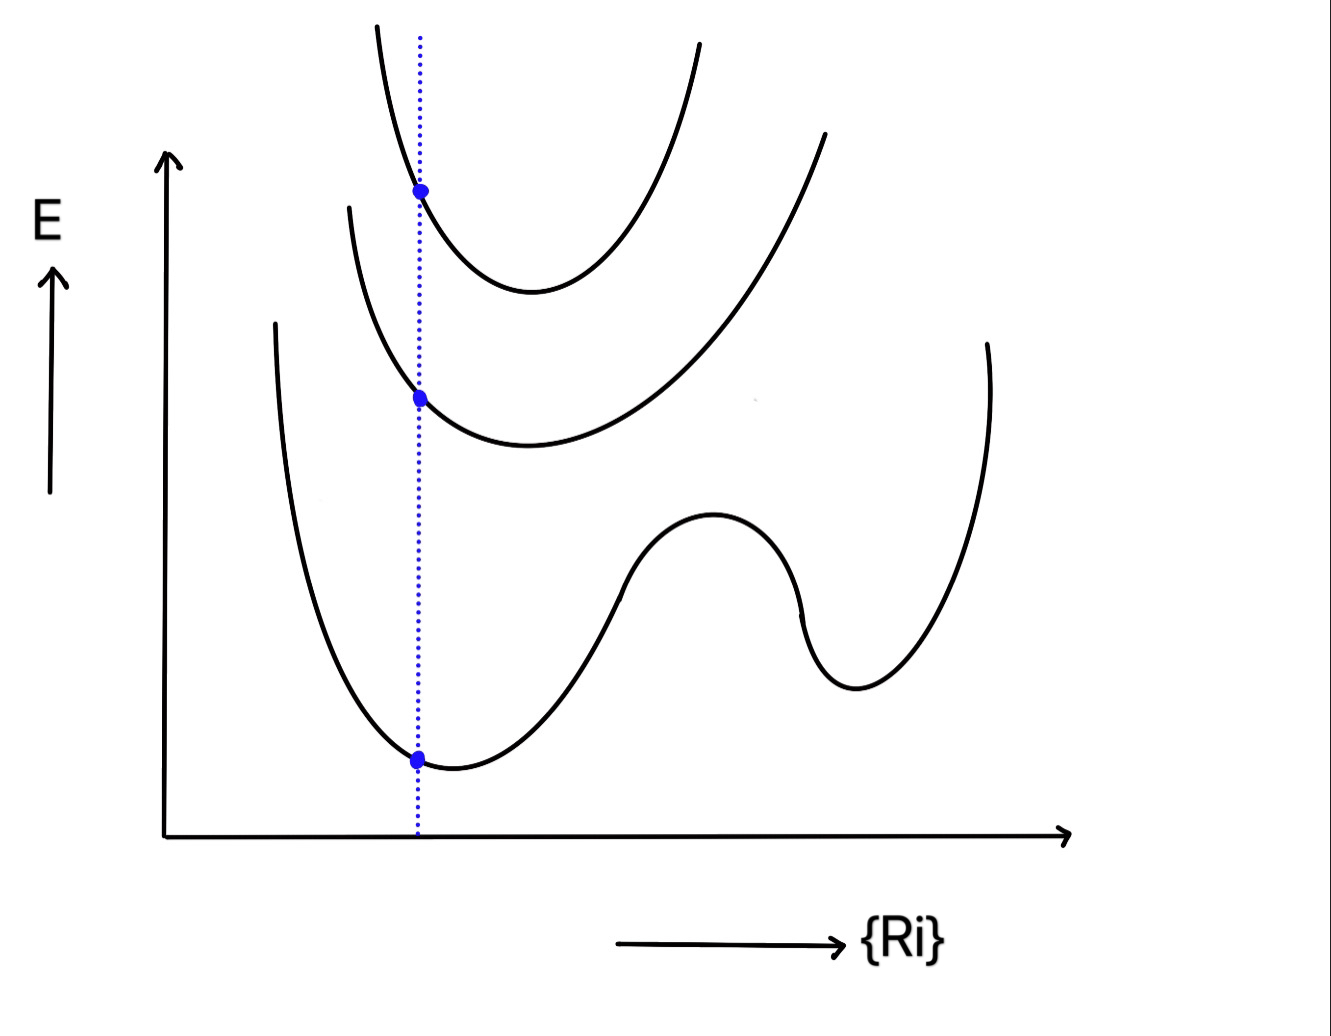
\includegraphics[width=.3\linewidth]{02.PNG}
        \caption{H-bonding among Water Molecules}
        \label{fig:sub-first2}
\end{figure}
Calculations in Gaussian:\\
\tab Put occupied orbitals for water molecule.
\begin{figure}[H]
        \centering
        % 1
        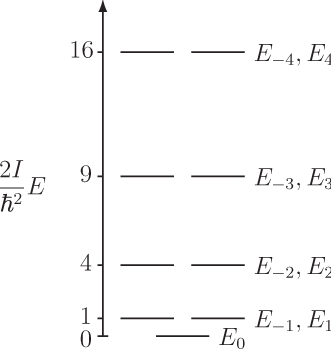
\includegraphics[width=.7\linewidth]{03.PNG}
        \caption{Four Occupied Orbitals of Water (Image from Anna Krylov)}
        \label{fig:sub-first2}
\end{figure}
\tab These are canonical MO's from Gaussian. They reflect the symmetry of water molecules, like symmetry or antisymmetry under point group operations.

\tab These things are very helpful to analyze the structure of water molecule. 


\item Example for localized VS delocalized: \\
	\tab Molecular orbital theory accounts for these observations with the concept of delocalized π bonds. In this picture, the four $2p_z$ orbitals are all parallel to each other (and perpendicular to the plane of the  $\sigma$  bonds). The four atomic ( $2p_z$ ) orbitals have combined to form four canonical MO's (delocalized over the whole molecule).
	\begin{figure}[H]
        \centering
        % 1
        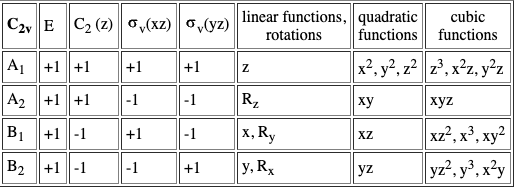
\includegraphics[width=.7\linewidth]{04.PNG}
        \caption{Delocalized Orbitals of the 1,3-butadiene Molecule (Image from \href{https://chem.libretexts.org/Bookshelves/General_Chemistry/Map\%3A_General_Chemistry_(Petrucci_et_al.)/11\%3A_Chemical_Bonding_II\%3A_Additional_Aspects/11.6\%3A_Delocalized_Electrons\%3A_Bonding_in_the_Benzene_Molecule}{Delocalized Electrons})}
        \label{fig:sub-first2}
\end{figure}
For computations:
\begin{itemize}
\item[a)] Localized orbitals are much more efficient for large molecules, because neglect long-range Coulomb interactions (approximation). 
\item[b)] Correlated with the Coupled Cluster method by using localized orbitals.
\end{itemize}
\end{itemize}


\begin{summary}{}{}
Density matrix is a crucial concept of Hartree-Fock theory. Here is a broad outline of density matrix:
\begin{itemize}
\item Discuss orbitals of water (non-unique).
\item Use of localized orthonormal orbitals VS delocalized.
\item Density matrix, $D$, can be associated with projection operator:
\begin{center}
		$\hat{D}=\sum_{a\in occ}|a\rangle \langle a|$ 
	\end{center}
$\hat{D}$ in HF projects on the space of occupied orbitals. The properties of orthogonal projection operator, $\hat{D}$:
\begin{center}
		$\hat{D}\hat{D}=\hat{D} \qquad \hat{D}^\dagger=\hat{D}$ 
	\end{center}
	$D_{\alpha\beta}$ in the non-orthogonal AO basis:
	\begin{center}
	$D_{\alpha\beta} = \langle \alpha|\hat{D}|\beta\rangle$\\
		$DSD=D$ 
	\end{center}
	In practice, we use AO basis. Details are more cumbersome, but basic properties are the same.
\end{itemize}

\end{summary}

\subsection{Derivation of Hartree-Fock Equations}
The energy of Hartree-Fock and the density matrix:
	\begin{IEEEeqnarray}{rLl}
E_{HF} &= \sum_{\mu,\nu} h_{\mu \nu} D_{\nu \mu} + \frac{1}{2}\sum_{\mu,\nu,\sigma,\tau}\langle \mu\nu||\sigma\tau\rangle D_{\sigma \mu}D_{\tau \nu} \\
D_{\nu\mu} &= \sum_{a,occ} C^*_{\mu a} C_{\nu a}  
	\end{IEEEeqnarray}
\tab The orthonormality: 
	\begin{IEEEeqnarray}{rLl}
\sum_{a,occ} C^*_{\mu a} S_{\mu\nu} C_{\nu b} &=\delta_{ab}
	\end{IEEEeqnarray}

Let us assume in the derivation that the orbitals (and integrals) are real. They are for molecules, not for solids. We want to optimize the energy, i.e $C_{\mu a}$, while preserving orthonormality of orbitals.

Define functional:
	\begin{IEEEeqnarray}{rLl}
F &= \sum_{\mu,\nu} h_{\mu \nu} D_{\nu \mu} + \frac{1}{2}\sum_{\mu,\nu,\sigma,\tau}\langle \mu\nu||\sigma\tau\rangle D_{\sigma \mu}D_{\tau \nu}- \sum_{a,b}\varepsilon_{ba} (\sum_{\mu,\nu} C^*_{\mu a} S_{\mu\nu} C_{\nu b} -\delta_{ab})
	\end{IEEEeqnarray}
\tab The $\varepsilon_{ab}$ are Lagrange multipliers, they allow us to do unconstraint variations of coefficients. We want: 
\begin{doublespace}
\begin{itemize}
	\item[1)] $\frac{\partial F}{\partial C_{\lambda d}}=0 \qquad \forall d,\lambda$
	\item[2)] $\frac{\partial F}{\partial \varepsilon _{ba}}=0 \Longrightarrow \sum_{\mu\nu} C^*_{\mu a} S_{\mu\nu} C_{\nu b} =\delta_{ab}$\\
	$\Longrightarrow$ constraints \\
	At convergence, $F=E$ is optimal. 
		\begin{IEEEeqnarray}{rLl}
\frac{\partial F}{\partial C_{\lambda d}}= \underbrace{ \sum_{\mu,\nu} h_{\mu \nu} \frac{\partial D_{\nu \mu} }{\partial  C_{\lambda d}} }_{A} + \underbrace{ \frac{1}{2}\sum_{\mu,\nu,\sigma,\tau}\langle \mu\nu||\sigma\tau\rangle \frac{\partial D_{\sigma \mu} }{\partial  C_{\lambda d}} D_{ \nu\tau} }_{B} + \underbrace{ \frac{1}{2}\sum_{\mu,\nu,\sigma,\tau}\langle \mu\nu||\sigma\tau\rangle D_{\sigma \mu} \frac{\partial D_{\nu\tau} }{\partial  C_{\lambda d}}  }_{C} \notag \\ \tab  -\underbrace{ \sum_{a,b}\varepsilon_{ba}\frac{\partial}{\partial C_{\lambda d}} (\sum_{\mu,\nu} C_{\mu a} S_{\mu\nu} C_{\nu b} -\delta_{ab})}_{D}
	\end{IEEEeqnarray}
\end{itemize}	
\end{doublespace}
	To simplify the equation(18) let me first note: 
\begin{itemize}
	\item The term $B$ is equal to the term $C$ in equation(18) by renaming indices of summation.\\
	Replace $\mu, \nu, \sigma, \tau$ by $\nu',\mu',\tau',\sigma'$
	\begin{IEEEeqnarray}{rLl}
\frac{1}{2}\sum_{\mu,\nu,\sigma,\tau}\langle \mu\nu||\sigma\tau\rangle D_{\sigma \mu} \frac{\partial D_{\nu\tau} }{\partial  C_{\lambda d}} &= \frac{1}{2}\sum_{\mu',\nu',\sigma',\tau'}\langle \nu'\mu'||\tau'\sigma'\rangle D_{\tau' \nu'} \frac{\partial D_{\sigma'\mu'} }{\partial  C_{\lambda d}} \notag \\
&= \frac{1}{2}\sum_{\mu',\nu',\sigma',\tau'}\langle \mu' \nu'||\sigma'\tau'\rangle\frac{\partial D_{\sigma'\mu'} }{\partial  C_{\lambda d}}  D_{\tau' \nu'} 
	\end{IEEEeqnarray}
	Don't need to drop the prime on indices (summation labels) and we have term B.
\item For the term A:
	\begin{IEEEeqnarray}{rLl}
\frac{\partial D_{\nu \mu} }{\partial  C_{\lambda d}} &= \frac{\partial}{\partial C_{\lambda d}}\sum_a(C_{\mu a}C_{\nu a}) \notag \\
&= \sum_a (\delta_{\mu\lambda}\delta_{ad}C_{\nu a}+C_{\mu a}\delta_{\nu \lambda}\delta_{ad} ) \notag \\
&= \delta_{\mu\lambda}C_{\nu d}+\delta_{\nu \lambda}C_{\mu d} \\
\frac{\partial D_{\sigma \tau} }{\partial  C_{\lambda d}} &= \delta_{\sigma\lambda}C_{\tau d}+ \delta_{\tau\lambda}C_{\sigma d}
	\end{IEEEeqnarray}
\tab NOTE:\\
\tab\tab The derivative of molecular orbitals: 
	\begin{IEEEeqnarray}{rLl}
\frac{\partial C_{\mu a}}{\partial C_{\lambda d}} = \delta_{\mu \lambda}\delta_{ad}
	\end{IEEEeqnarray}
	\tab They are independent coefficients. All derivatives are zero, expect the derivative is 1 when $\mu=\lambda, a=d$.
\item For the term D:
	\begin{IEEEeqnarray}{rLl}
\frac{\partial}{\partial C_{\lambda d}} (\sum_{a,b}\varepsilon_{ba} \sum_{\mu,\nu} C_{\mu a} S_{\mu\nu} C_{\nu b} -\delta_{ab}) &= \sum_{\mu,\nu}\sum_{a,b}\varepsilon_{ba} (\delta_{\mu\lambda}\delta_{ad}S_{\mu\nu}C_{\nu b}+C_{\mu a}S_{\mu\nu}\delta_{\nu\lambda}\delta_{bd} ) \notag \\
&= \sum_{\nu b}S_{\lambda \nu}C_{\nu b}\varepsilon_{bd}+\sum_{a \mu}C_{\mu a}S_{\mu\lambda}\varepsilon_{da}
	\end{IEEEeqnarray}
\end{itemize}
This leads to: 
	\begin{IEEEeqnarray}{rLl}
&\sum_{\mu,\nu} h_{\mu \nu} \delta_{\mu\lambda}C_{\nu d}+ \sum_{\mu,\nu} h_{\mu \nu}\delta_{\lambda \nu}C_{\mu d}+\sum_{\mu,\nu,\sigma,\tau}\langle \mu\nu||\sigma\tau\rangle D_{\nu \tau} (\delta_{\mu\lambda}C_{\nu d}+\delta_{\nu \lambda}C_{\mu d}) \notag \\
&- S_{\lambda \nu}C_{\nu b}\varepsilon_{db} -S_{\lambda \nu}C_{\lambda a}\varepsilon_{ad} = 0
	\end{IEEEeqnarray}
Or: 
	\begin{IEEEeqnarray}{rLl}
&\left[ \sum_\nu h_{\lambda\nu}C_{\nu d}+ \sum_{\sigma\tau}\langle \lambda\nu||\sigma\tau\rangle D_{\nu \tau}C_{\sigma d} - S_{\lambda\nu}C_{\nu b}\varepsilon_{bd}^* \right] \notag \\
+& \left[ \sum_{\mu}C_{\mu d}h_{\mu \lambda}+\sum_{\nu,\tau}C_{\mu d}\langle \mu\nu||\lambda\tau\rangle D_{\nu\tau}-\varepsilon_{da}^*C_{\lambda a}S_{\lambda \nu}  \right] =0
	\end{IEEEeqnarray}
If we now define the so-called Fock matrix in AO basis, $f$:
	\begin{IEEEeqnarray}{rLl}
f_{\mu \sigma} = \sum_{\nu \tau}\langle \mu\nu||\sigma\tau\rangle D_{\nu \tau}+ h_{\mu\sigma}
	\end{IEEEeqnarray}
We can write: 
	\begin{IEEEeqnarray}{rLl}
\sum_\nu f_{\lambda \nu}C_{\nu d} -\sum_{\nu,b}S_{\lambda \nu}C_{\nu b}\varepsilon_{bd}+ \sum_{\mu}C_{\mu d}f_{\mu \lambda}- \sum_{a,\lambda}\varepsilon_{da}C_{\lambda a}S_{\lambda \nu} &=0 \\
(fC-SC\varepsilon )+(C^\dagger f - \varepsilon C^\dagger S )&=0 \\
(fC-SC\varepsilon )+(fC-  SC\varepsilon^\dagger )^\dagger &=0 
	\end{IEEEeqnarray}
If we assume (can be shown) that $\varepsilon = \varepsilon^\dagger$, then:
	\begin{IEEEeqnarray}{rLl}
fC-  SC\varepsilon &=0 
	\end{IEEEeqnarray}
Here $\varepsilon$ is a matrix of Lagrange multipliers. If  $\varepsilon = \varepsilon^\dagger$, it can be diagonalized. ($\lambda$ is diagonal)
	\begin{IEEEeqnarray}{rLl}
\varepsilon &= u \lambda u^\dagger \\
\varepsilon u &= u \lambda \\
\Longrightarrow f(Cu) &= S(Cu)\lambda  \\
fC' &= SC'\lambda
	\end{IEEEeqnarray}
Note that $C'$ are the so-called canonical orbitals.\\
 They satisfy the generalized eigenvalue equation.
	\begin{IEEEeqnarray}{rLl}
fC &= SC\lambda \notag \\
&= SC\varepsilon
	\end{IEEEeqnarray}
Note that $\varepsilon$ is diagonal matrix. 


As we have shown before, the density matrix is invariant under transformation of occupied orbitals. The orbitals that we obtain from Hartree-Fock, are usually canonical orbitals, together with Hartee-Fock orbital energies. The derivation of Hartree-Fock equations is difficult. We are also obtaining equations that are not so easy to interpret. Let me try to clarify in a next set of notes.
	



















\end{document}